\documentclass[implementacija.tex]{subfiles}
\usepackage{subfiles}
\documentclass[12pt,oneside]{memoir} 
\usepackage[latinica]{matfmaster} 

\begin{document}

Projekat je realizovan iz dva projekta čija su imena \textit{GC STT Remote} (u nastavku: gugl aplikacija) i \textit{Basic Mic Remote} (u nastavku: osnovna aplikacija). Kako su ova dva projekta u velikoj većini ista prvo će biti obuhvaćen pregled svih fajlova koji su isti i čine temelj aplikacije. Zatim će detaljnije biti objašnjeno sve vezano za upotrebu mikrofona. 

Osnovnu strukturu \textbf{app} direktorijuma bilo koje Android aplikacije čine poddirektorijumi: 

\begin{itemize}
\item \textit{build} sa izvršnom verzijom k\^{o}da ,
\item \textit{libs} sa eksternim bibliotekama odnosno bibliotekama koje nisu deo Androida, Java ili Kotlin programskih jezika i
\item \textit{src} sa izvornim k\^{o}dom.
\end{itemize}

% //TODO
 % Dodati link tj. clickable ka svakom opisu tj. podnaslovu
 Direktorijum \textbf{src} se uglavnom sastoji od sledečih poddiretkorijuma: 
\begin{itemize}
\item \textit{AndroidTest} u kom se smeštaju svi testovi koje je potrebno pokrenuti na Android uređaju, 
\item \textit{test} u kom se smeštaju svi testovi za testiranje jedinica k\^{o}da (eng. \textit{unit tests})
\item \textit{main} u kom se nalazi ceo izvorni k\^{o}d.
\end{itemize}

Srž aplikacije se nalazi u \textbf{main} direktorijumu. Za aplikaciju koju opisujemo ovaj direktorijum ima sledeću strukturu:
\begin{itemize}
\item \textit{AndroidMainifest.xml} - datoteka koji opisuje glavne postavke aplikacije,
\item \textit{res} - direktorijum sa svim XML datotekama koje čine korisnički interfejs (eng. \textit{user interface}) aplikacije,
\item \textit{java} - direktorijum sa svim klasama i interfejsima aplikacije
\item \textit{proto} - direktorijum sa \textit{.proto} datotekama koje su neophodne za korišćenje \textit{Google Cloud API}-ja. Ovaj folder se nalazi samo u gugl aplikaciji.
\end{itemize}

%TODO
% Opisati build.gradle -> oba fajla
Važne datoteke pri postavljanju projekta su \textit{build.gradle} datoteke koje služe da  upravljaju procesom izgradnje i odrede zavisnosti (eng. \textit{dependency}) aplikacije. Postoje dva tipa ovih datoteka - na nivou projekta i na nivou modula. <<TODO: Raspisati o ovim datotekama>>

\section{AndroidManifest aplikacije}

Informacije potrebne za pokretanje i instalaciju aplikacije čine AndroidManifest.xml datoteku. U ovoj datoteci su definisane sve dozvole koje su potrebne da budu dozvoljene na uređaju sa kog se pokreće aplikacija: pristup internetu, wifi stanju, stanju telefona, vibracija i  snimanje audio sadržaja. Pregled ovih dozvola je dat u listingu \ref{lst:manifestApp}. U okviru etiketa (eng. \textit{tag}) koji definiše aplikaciju su postavljene vrednosti naziva aplikacije, slika kojom je aplikacija predstavljena, ciljani API nivo kao i dve aktivnosti koje se pojavljuju. Prva aktivnost je \textit{ChooseConnection}, koja je odabir uređaja sa kojim će se korisnik povezati i ona je obeležena kao glavna aktivnost. Druga aktivnost je \textit{RemoteView} koja čini prikaz daljinskog upravljača. 

\lstinputlisting[language=XML, caption= {Odobrenja definisana u AndroidManifest.xml fajlu}, label={lst:manifestApp}]{AppManifest.xml}


\section{Direktorijum res}
Direktorijum u kom se smeštaju svi resursi aplikacije se naziva \textit{res}. Resursi koji se mogu čuvati su slike, planovi (eng. layout), stringovi, stilovi itd. Moguće je čuvati iste resurse u različitim dimenzijama kako bi u zavisnosti od dimenzija i podešavanja uređaja bile odabrane adekvatne dimenzije. \textit{Drawable} direktorijum skladišti slike. Za potrebe projekta formirane su i sačuvane slike za strelicu koja je predstavljena trouglom, ovalno dugme i dugme za prekid konekcije. 

Vrednosti, boje i dimenzije za različite resurse se skladište u \textit{values} direktorijumu. Datoteka \textit{colors.xml} sadrži boje korišćene za kreiranje interfejsa. Stringovi potrebni za dizajn korisničkog interfejsa su sačuvani u \textit{strings.xml}. Kolor shema, odnosno tema aplikacije je definisana u \textit{themes/themes.xml} odakle se može uočiti da boje koje se koriste za korisnički interfejs su nijanse plave boje. 

Svaki ekran sa kojim se korisnik može susresti mora imati korisnički interfejs koji ima svoj plan opisan unutar XML datoteke. Skup svih planova je smešten unutar \textit{layout} direktorijuma koji u primeru ove aplikacije ima sledeće XML datoteke:
\begin{itemize}
\item \textbf{activity\_choose\_stb} predstavlja plan ekrana za odabir konekcije, odnosno stb uređaja sa kojim korisnik želi da se poveže. Ovaj plan je kreiran pomoću klase \textit{RelativeLayout}. Unutar \textit{RelativeLayout}-a nalaze se tri komponente koje se mogu prikazati ili skloniti u zavisnosti od potrebe. Prva komponenta je \textit{RecyclerView} sa id-jem \textit{@+id/rv\_boxes\_list} sa podešenom vidljivošću na \textit{gone} što znači da je inicijalno skriven. Njegova vidljivost se menja u k\^{o}du u trenutku kada se pronađu uređaji na mreži tako što se postavlja na \textit{visible}, odnosno da je vidljiv. Sledeća komponenta je \textit{ProgressBar} koji može poslužiti prilikom učitavanja. Poslednja komponenta je \textit{RelativeLayout} sa id-jem \textit{@+id/rl\_pairing\_container} koji je inicijalno sakriven. On sadrži tekstualno polje tipa \textit{TextView} sa uputstvom korisniku da unese k\^{o}d koji vidi na ekranu uređaja sa kojim pokušava uparivanje, polje za unos teksta tipa \textit{EditText} u koji se unosi k\^{o}d i dugme za potvrdu unosa. Ceo ovaj plan postaće vidljiv kada korisnik odabere uređaj sa kojim želi da se poveže. Izgled ovog plana može se videti na slici <<dodaj sliku>>.
\item \textbf{remote\_control\_scene} - Ovaj plan predstavlja izgled daljinskog upravljača. Sve komponente su unutar \textit{ConstraintLayout}-a koji omogućava da udaljenost komponenti bude predstavljena ograničenjima (eng. constraint). Korisnički interfejs ovog plana kao i shematski plan zajedno sa svim ograničenjima se može videti na slici \ref{fig:remoteScena}. Dugmići za paljenje/gašenje uređaja, prekid konekcije sa povezanim uređajem, vraćanje nazad, gašenje zvuka i mikrofon su objekti tipa \textit{ImageButton}. Svi ostali dugmići su kreirani pomoću klase \textit{Button}. Nad svim dugmićima je postavljena opcija da se na pritisak dugmeta pozove metoda \textit{onClick()}. O akcijama koje se dese prilikom pritiska dugmeta i poziva metode \textit{onClick} biće reči u nastavku poglavlja. U prvom nizu su dugmići za paljenje/gašenje uređaja, zatim dugme \textit{GUIDE} koje prikazuje elektronski vodič kroz program (eng. \textit{Electronic Program Guide (EPG)}) i na kraju dugme za prekid konekcije između uređaja. Dugmići za brojeve su podeljeni u četiri horizontalna \textit{LinearLayout}-a sa po tri dugmeta. Poslednji od njih sadrži i dugme \textit{MOVIE} koje prikazuje obabir filmova za iznajmljivanje i dugme \textit{LIVE} koje prebacuje ekran na sadržaj koji je uživo na tv-u. Centralni deo ekrana zauzima dugme za potvrdu izbora \textit{OK} i strelice za levo, desno, gore i dole. Strelice su kreirane samostalno i u implementaciji je zato potrebno dodati  \verb|android:background="@drawable/arrow"|. Dugmići za povratak na prethodno prikazano, mikrofon i \textit{HOME} - prikaz početnog ekrana su grupisani u jedan \textit{LinearLayout}. Na samom dnu ekrana se nalazi još jedan \textit{LinearLayout} koji se sastoji od dva vertikalna \textit{LinearLayout}-a, za menjanje kanala i podešavanje jačine zvuka. Između njih je dugme za totalno gašenje zvuka.  
\item \textbf{stb\_view} - Ovaj plan je jedan \textit{RelativeLayout} koji čini samo jedan \textit{TextView}. Prikazuje se onda kada je potrebno prikazati imena stb-ova koji su pronađeni. Inicijalno nema nikakav tekst.
\end{itemize}

%=================== SLIKA ======================================
\begin{figure}[!ht]
  \centering
  \label{fig:remoteScena}
  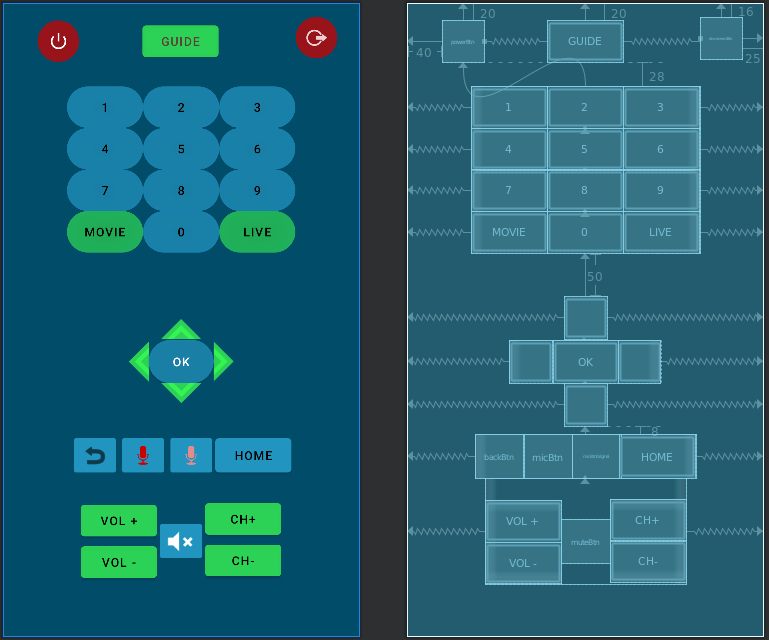
\includegraphics[width=\textwidth]{Implementacija/remote_control_scene.png}
  \caption{Korisnički interfejs i shematski plan daljinskog upravljača}
\end{figure}
%=====================================================================

% opisati sve ove fajlove koje imam

\section{Direktorijum java}
Za funkcionisanje aplikacije neophodno je da se omogući pronalaženje uređaja, a zatim i da se manipuliše sa odabranim uređajem. Kako bi ovo sve radilo ispravno potrebna je međusobna interakcija između klasa, kao i podela k\^{o}da u adekvatne pakete i klase prema funkcionalnostima koje obezbeđuju. Iz tih razloga unutar glavnog paketa aplikacije k\^{o}d je podeljen u dva paketa. Paket \textit{stbs} sadrži klase koje se bave pronalaženjem i upravljanjem stb-om. Klase koje se bave upravljanjem komandama i komunikacijom sa uređajem su smeštene u paket \textit{controller}. 

Klase unutar \textbf{stbs} paketa su:
\begin{itemize}
\item \textit{ChooseAdapter} koja se koristi za prikaz liste pronađenih uređaja,
\item \textit{ChooseConnection} koja se koristi za odabir i povezivanje sa izabranim uređajem,
\item \textit{DiscoveryHandler} se koristi za pronalaženje dostupnih uređaja u mreži,
\item \textit{NsdDiscover} koja se koristi za korišćenje NSD (eng. \textit{Network Service Discovery}) mehanizma za pronalaženje uređaja i
\item \textit{Stb} koja predstavlja jedan uređaj i sadrži informacije o njemu.
\end{itemize}


Klase unutar \textbf{controller} paketa su:
\begin{itemize}
\item \textit{CommandsHandler} koja je odgovorna za obradu i slanje komandi na uređaj,
\item \textit{RemoteView} koja se bavi prikazom i interakcijom korisnika sa aplikacijom,
\item \textit{UdpClient} koja omogućava komunikaciju putem UDP protokola i
\item \textit{StreamingRecognizeClient} koje se koristi u GC verziji za obradu audio podataka i prepoznavanje govora. 
\end{itemize}


Pored ovih klasa u glavnom paketu aplikacjie nalaze se sledeće klase i interfejsi:
\begin{itemize}
\item \textit{AsyncDataReceiver} interfejs služi za primanje asinkronih podataka,
\item \textit{AsyncReceiver} interfejs služi za primanje asinhronih podataka,
\item \textit{OnItemClickedListener} interfejs služi za obradu klikova na elemente liste,
\item \textit{Singleton} klasa se koristi za implementaciju Singlton (eng. \textit{Singleton}) šablona i
\item \textit{Constants} klasa koja skladišti sve konstante potrebne u razvoju.
\end{itemize}

\subsection{Stbs paket}
\subfile{stbs}

\subsection{Controller paket}
\subfile{controller}

\subsection{Klase iz glavnog paketa}

\section{Direktorijum proto}



% slika podele koda src -> Manifets, res, com, proto + gradle
% Manifest sta ima, glavni delovi
% gradle kako je podesen
% res folder, ukratko xml implementacije neki specif. stvari
% com folder -> tu imamo 2 paketa + ovi glavni
% proto kad i zasto je koriscen
\end{document}